\FloatBarrier
\begin{figure}[!h]
\centering
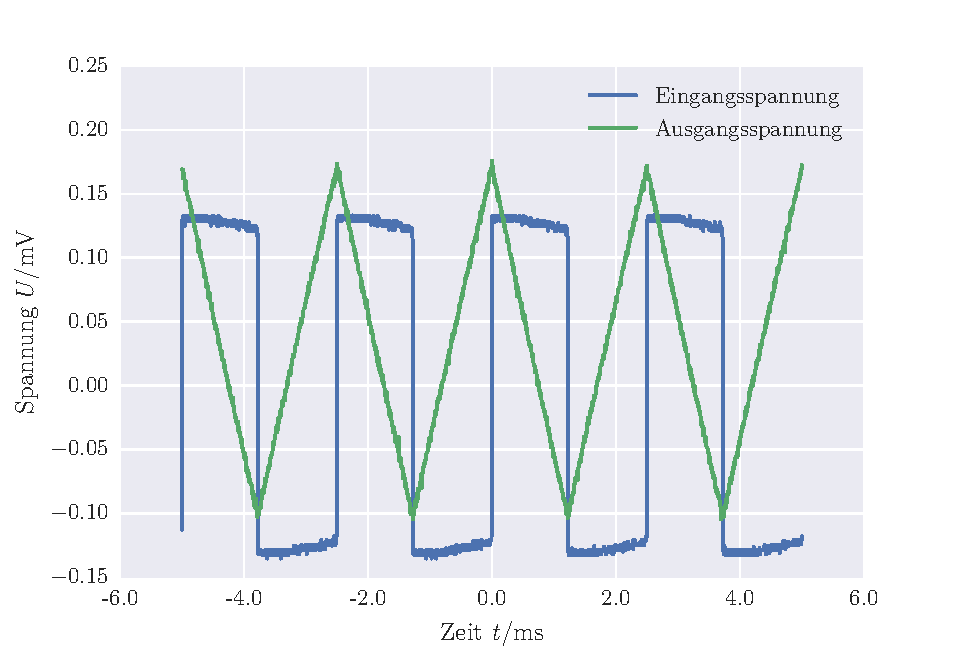
\includegraphics[scale=0.75]{../Grafiken/Integrator_Oszilloskop_Rechteck.pdf}
\caption{Vom Oszilloskop aufgenommene Ein- und Ausgangsspannungen der Integratorschaltung. Auf dem Eingang
	liegt hier eine Rechteckspannung.  Die Ausgangsspannung in Form einer Dreieckspannung entspricht dem theoretisch
	zu erwartendem Verlauf.\label{fig:integrator_oszilloskop_rechteck}}
\end{figure}
\FloatBarrier